\documentclass[aspectratio=169,11pt]{beamer}
\usepackage[T1]{fontenc}
\usepackage{lmodern}
\usepackage{amsmath,amssymb,mathtools}
\usepackage{booktabs}
\usepackage{tikz}
\usetikzlibrary{arrows.meta,positioning,calc,decorations.pathmorphing}

\definecolor{ink}{HTML}{1B2A41}
\definecolor{accent}{HTML}{C8551B}
\definecolor{soft}{HTML}{EEF2F7}
\setbeamercolor{frametitle}{fg=white,bg=ink}
\setbeamercolor{normal text}{fg=ink}
\setbeamercolor{structure}{fg=accent}
\setbeamercolor{block title}{fg=white,bg=ink}
\setbeamercolor{block body}{bg=soft}
\setbeamerfont{frametitle}{size=\large,series=\bfseries}
\setbeamertemplate{navigation symbols}{}
\setbeamertemplate{itemize items}{\color{accent}$\blacktriangleright$}
% Dark band at the bottom reserved for burned-in subtitles.
\setbeamertemplate{footline}{%
  \begin{tikzpicture}[remember picture,overlay]
    \fill[ink] (current page.south west) rectangle ([yshift=11mm]current page.south east);
  \end{tikzpicture}\vspace*{11mm}}
\setbeamertemplate{frametitle}{%
  \nointerlineskip
  \begin{beamercolorbox}[wd=\paperwidth,ht=8mm,dp=3mm,leftskip=5mm,rightskip=5mm]{frametitle}
    \insertframetitle\hfill{\scriptsize\mdseries JSP-000005 \textperiodcentered{} Exposition \textperiodcentered{} \insertframenumber/\inserttotalframenumber}
  \end{beamercolorbox}}

\newcommand{\R}{\mathbb{R}}
\newcommand{\Res}{\mathcal{R}}
\newcommand{\src}[1]{{\scriptsize\color{accent}\textsf{[#1]}}}

\begin{document}

% 1 -------------------------------------------------------------
{\setbeamertemplate{footline}{%
  \begin{tikzpicture}[remember picture,overlay]
    \fill[ink] (current page.south west) rectangle ([yshift=11mm]current page.south east);
  \end{tikzpicture}\vspace*{11mm}}
\begin{frame}[plain]
\vspace{4mm}
\begin{center}
{\color{accent}\small JUSTIN SUN PRIZE \textperiodcentered{} JSP-000005 \textperiodcentered{} EXPOSITION}\\[5mm]
{\LARGE\bfseries How a Forced Navier--Stokes Flow Blows Up}\\[3mm]
{\normalsize A guided tour of OpenAI's finite-time blowup construction}\\[7mm]
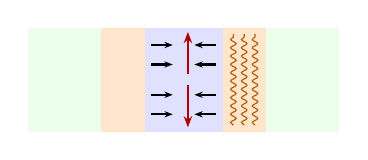
\begin{tikzpicture}[scale=0.55]
 \fill[blue!12] (-0.9,-1.2) rectangle (0.9,1.2);
 \fill[orange!20] (0.9,-1.2) rectangle (1.9,1.2); \fill[orange!20] (-1.9,-1.2) rectangle (-0.9,1.2);
 \fill[green!8] (1.9,-1.2) rectangle (3.6,1.2); \fill[green!8] (-3.6,-1.2) rectangle (-1.9,1.2);
 \foreach \y in {-0.8,-0.35,0.35,0.8}{\draw[-{Stealth[length=3pt]},thick] (0.75,\y)--(0.25,\y);\draw[-{Stealth[length=3pt]},thick] (-0.75,\y)--(-0.25,\y);}
 \draw[-{Stealth[length=4pt]},thick,red!70!black] (0.1,0.12)--(0.1,1.1);
 \draw[-{Stealth[length=4pt]},thick,red!70!black] (0.1,-0.12)--(0.1,-1.1);
 \foreach \x in {1.15,1.4,1.65}{\draw[orange!70!black,decorate,decoration={snake,amplitude=1pt,segment length=3pt}] (\x,-1.05)--(\x,1.05);}
\end{tikzpicture}\\[6mm]
{\small Thanh Van Nguyen \quad\textperiodcentered\quad Companion video to the essay (v1.0, 29 October 2026)}\\[1mm]
{\scriptsize All mathematics is due to the authors of the source paper. This is an exposition.}
\end{center}
\end{frame}}

% 2 -------------------------------------------------------------
\begin{frame}{The question: Navier--Stokes in three dimensions}
\[
\partial_t u+(u\cdot\nabla)u=\nu\Delta u-\nabla p+f,\qquad \nabla\cdot u=0,\qquad u(\cdot,0)=u^\circ
\]
\vspace{-2mm}
\begin{columns}[T]
\begin{column}{0.48\textwidth}
\begin{block}{Unforced ($f\equiv0$): global regularity}
\textbf{(A)} on $\R^3$\qquad \textbf{(B)} on the torus $\R^3/\mathbb Z^3$\\[1mm]
\small smooth solutions for all time, for all smooth data
\end{block}
\end{column}
\begin{column}{0.48\textwidth}
\begin{block}{Breakdown: a force is allowed}
\textbf{\color{accent}(C)} on $\R^3$\qquad \textbf{\color{accent}(D)} on the torus\\[1mm]
\small smooth data and force with \emph{no} global smooth bounded-energy solution
\end{block}
\end{column}
\end{columns}
\vspace{3mm}
\centering\small Fefferman, official Clay Millennium Problem statement. Proving any one alternative resolves the problem.
\end{frame}

% 3 -------------------------------------------------------------
\begin{frame}{The result \src{Paper, Theorem 1.1}}
\begin{block}{For every $\nu>0$ there exist}
a force $f\in C_c^\infty(\R^3\times(0,\infty))$ and smooth $u,p$ on $\R^3\times[0,1)$ with $u(\cdot,0)=0$,\\
supported in a fixed compact set $K$, such that
\[
\sup_{t<1}\|u(t)\|_{L^2}<\infty,\qquad \limsup_{t\uparrow1}\|u(t)\|_{L^\infty}=\infty .
\]
\end{block}
\begin{itemize}
\item $\Rightarrow$ alternative \textbf{(C)}; rescaling + periodizing $\Rightarrow$ \textbf{(D)}
\item \textbf{Not} addressed: the unforced alternatives (A) and (B)
\item Status: Lean formalization released; independent peer review pending
\end{itemize}
\end{frame}

% 4 -------------------------------------------------------------
\begin{frame}{Why three dimensions are hard \src{Context}}
\begin{columns}[T]
\begin{column}{0.47\textwidth}
Scaling symmetry
\[
u_\lambda(x,t)=\lambda\,u(\lambda x,\lambda^2t)
\]
Energy under zoom-in:
\[
\|u_\lambda\|_{L^2}^2=\lambda^{-1}\|u\|_{L^2}^2
\]
\small Small scales weaken the only global bound\\ $\Rightarrow$ energy is \textbf{supercritical}.
\end{column}
\begin{column}{0.5\textwidth}
\small
\begin{itemize}
\item 1934 Leray: global weak solutions
\item 1982 Caffarelli--Kohn--Nirenberg: small singular set
\item 2003 Escauriaza--Seregin--\v{S}ver\'ak: $L^\infty L^3$ regularity
\item 2016 Tao: blowup for an \emph{averaged} equation
\item 2019--22 Buckmaster--Vicol, Albritton--Bru\'e--Colombo: non-uniqueness
\item 2023--26 C\'ordoba--Mart\'inez-Zoroa(--Zheng): forced Euler / hypodissipative blowup
\end{itemize}
\end{column}
\end{columns}
\end{frame}

% 5 -------------------------------------------------------------
\begin{frame}{Key reformulation: choose the flow, read off the force}
\[
\Res(u,p):=\partial_t u+(u\cdot\nabla)u-\nu\Delta u+\nabla p \qquad\Longrightarrow\qquad f:=\Res(u,p)
\]
\begin{block}{The real problem}
Design $(u,p)$ that blows up at $t=1$ while $\Res(u,p)$ \textbf{and all its derivatives} extend smoothly through $t=1$.
\end{block}
\vspace{2mm}
Flatness \src{Paper, eq.~(3.4)}:
\[
|\partial_x^\alpha\partial_t^b\,\Res(u,p)|\le C_{\alpha,b,N}\,q^N\qquad\text{for every }N,
\]
\small $q\to0$ measures the distance to the singular point. Each term blows up; their sum must cancel to infinite order.
\end{frame}

% 6 -------------------------------------------------------------
\begin{frame}{The collapsing vortex \src{Paper, \S2}}
\begin{columns}[c]
\begin{column}{0.56\textwidth}
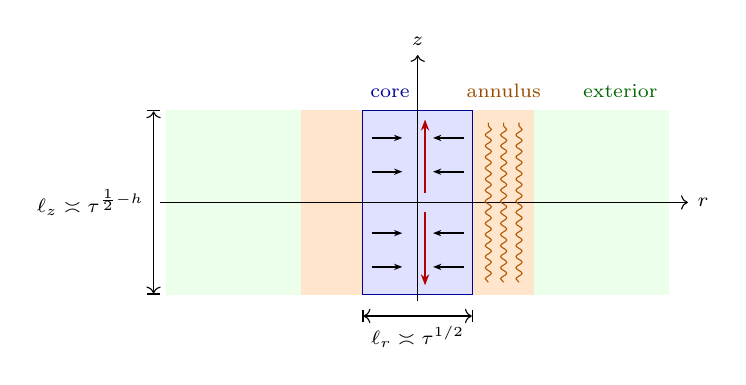
\begin{tikzpicture}[scale=0.78]
 \fill[blue!12] (-0.9,-1.5) rectangle (0.9,1.5);
 \draw[blue!60!black] (-0.9,-1.5) rectangle (0.9,1.5);
 \fill[orange!20] (0.9,-1.5) rectangle (1.9,1.5); \fill[orange!20] (-1.9,-1.5) rectangle (-0.9,1.5);
 \fill[green!8] (1.9,-1.5) rectangle (4.1,1.5); \fill[green!8] (-4.1,-1.5) rectangle (-1.9,1.5);
 \draw[->] (-4.2,0)--(4.4,0) node[right]{\scriptsize $r$};
 \draw[->] (0,-1.6)--(0,2.4) node[above]{\scriptsize $z$};
 \node[blue!60!black,anchor=south,font=\scriptsize] at (-0.45,1.55) {core};
 \node[orange!60!black,anchor=south,font=\scriptsize] at (1.4,1.55) {annulus};
 \node[green!40!black,anchor=south,font=\scriptsize] at (3.3,1.55) {exterior};
 \foreach \y in {-1.05,-0.5,0.5,1.05}{\draw[-{Stealth[length=3pt]},thick] (0.75,\y)--(0.25,\y);\draw[-{Stealth[length=3pt]},thick] (-0.75,\y)--(-0.25,\y);}
 \draw[-{Stealth[length=4pt]},thick,red!70!black] (0.12,0.15)--(0.12,1.35);
 \draw[-{Stealth[length=4pt]},thick,red!70!black] (0.12,-0.15)--(0.12,-1.35);
 \foreach \x in {1.15,1.4,1.65}{\draw[orange!70!black,decorate,decoration={snake,amplitude=1.1pt,segment length=4pt}] (\x,-1.3)--(\x,1.3);}
 \draw[|<->|] (-0.9,-1.85)--(0.9,-1.85) node[midway,below,font=\scriptsize]{$\ell_r\asymp\tau^{1/2}$};
 \draw[|<->|] (-4.3,-1.5)--(-4.3,1.5) node[midway,left,font=\scriptsize]{$\ell_z\asymp\tau^{\frac12-h}$};
\end{tikzpicture}
\end{column}
\begin{column}{0.42\textwidth}
\small
\begin{itemize}
\item $\tau=1-t$; cylindrical $(r,\theta,z)$
\item core: inward spiral, axial outflow
\item inflow conserves $ru_\theta$ $\Rightarrow$ spin-up; viscosity balances it
\item exterior: pure swirl solving the heat equation exactly, so zero residual
\item fixed $0<h<\tfrac1{100}$: radius shrinks faster than height
\end{itemize}
\end{column}
\end{columns}
\end{frame}

% 7 -------------------------------------------------------------
\begin{frame}{Scales of the core \src{Paper \S2.1, \S3.5; Check}}
\centering
\[
|u_\theta|,|u_z|\asymp\tau^{-\frac12-h},\qquad |u_r|=O(\tau^{-\frac12}),\qquad \text{volume}\asymp\tau^{\frac32-h}
\]
\small
\begin{tabular}{@{}lll@{}}
\toprule
Quantity & Scale & Meaning\\
\midrule
kinetic energy & $\tau^{1/2-3h}\to0$ & energy stays bounded\\
dissipation rate & $\tau^{-1/2-3h}$ & integrable since $h<1/6$\\
swirl Reynolds number & $\tau^{-h}\to\infty$ & many turns per diffusion time\\
radial Reynolds number & $O(1)$ & viscosity stays in the balance\\
$\sqrt{\tau}\,\|u\|_{L^\infty}$ & $\tau^{-h}\to\infty$ & faster than self-similar\\
\bottomrule
\end{tabular}
\end{frame}

% 8 -------------------------------------------------------------
\begin{frame}{The missing momentum is a stress in the annulus \src{Paper \S3.2}}
\[
R^{(0)}_\theta=-(\partial_r+\tfrac2r)\,T_{r\theta},\qquad R^{(0)}_z=-(\partial_r+\tfrac1r)\,T_{rz}
\]
\begin{itemize}
\item core and heat exterior balance their own momentum
\item the joining annulus $X_a<X<X_b$ leaves a residual that blows up
\item it is a \textbf{radial flux} of swirl and axial momentum: a stress $T$
\item matching \textbf{five radial integrals} keeps $T$ supported in the annulus
\item a small oscillation $\sim N^{-1}\sin(N\log X)$ steers the shear so that $T$ lies in the \textbf{admissible stress cone}
\end{itemize}
\end{frame}

% 9 -------------------------------------------------------------
\begin{frame}{Pulses supply the stress \src{Paper \S3.3; Heuristic}}
\begin{columns}[c]
\begin{column}{0.58\textwidth}
\[
\Res(u_B+w)=\Res(u_B)+L_{u_B}w+\nabla\cdot(w\otimes w)
\]
Plane wave $w=a\cos(\xi\cdot x+\varphi)$, $a\cdot\xi=0$:
\begin{itemize}\small
\item $\nabla\cdot w=0$ and $(w\cdot\nabla)w=0$
\item average stress $\langle w\otimes w\rangle=\tfrac12\,a\otimes a$
\item slowly varying amplitude $\Rightarrow$ prescribable force
\item squared amplitudes are positive, so two families reach exactly the cone $c_1v_1+c_2v_2$, $c_i>0$
\end{itemize}
\end{column}
\begin{column}{0.38\textwidth}
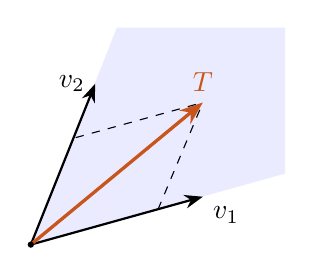
\begin{tikzpicture}[scale=0.95]
\fill[blue!8] (0,0)--(3.4,0.95)--(3.4,2.9)--(1.15,2.9)--cycle;
\draw[-{Stealth},thick] (0,0)--(2.3,0.64) node[below right]{$v_1$};
\draw[-{Stealth},thick] (0,0)--(0.86,2.15) node[left]{$v_2$};
\draw[dashed] (1.7,0.47)--(2.3,1.9); \draw[dashed] (0.6,1.43)--(2.3,1.9);
\draw[-{Stealth},very thick,accent] (0,0)--(2.3,1.9) node[above]{$T$};
\fill (0,0) circle (1.2pt);
\end{tikzpicture}
\end{column}
\end{columns}
\end{frame}

% 10 ------------------------------------------------------------
\begin{frame}{Where pulses get their energy \src{Heuristic; Paper \S2.2}}
\begin{columns}[c]
\begin{column}{0.52\textwidth}
Rayleigh's toy model for swirl $V(r)$:
\[
\ddot w_r=-\frac{k_z^2}{|k|^2}\,\kappa^2 w_r,\qquad \kappa^2=\frac1{r^3}\frac{d}{dr}(rV)^2
\]
\small
\begin{itemize}
\item angular momentum decreasing outward $\Rightarrow\kappa^2<0$ $\Rightarrow$ growth
\item shear tilts wave fronts, so $|k_r|$ grows
\item amplification weakens, damping $\nu|k|^2$ grows
\item each pulse rises, then decays
\end{itemize}
\end{column}
\begin{column}{0.44\textwidth}
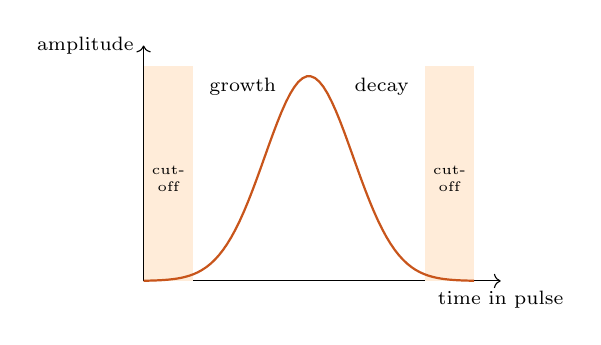
\begin{tikzpicture}[xscale=4.2,yscale=2.6]
\draw[->] (0,0)--(1.08,0) node[below]{\scriptsize time in pulse};
\draw[->] (0,0)--(0,1.15) node[left]{\scriptsize amplitude};
\fill[orange!15] (0,0) rectangle (0.15,1.05); \fill[orange!15] (0.85,0) rectangle (1,1.05);
\draw[thick,accent,domain=0:1,samples=80] plot (\x,{exp(-28*(\x-0.5)^2)});
\node[font=\scriptsize] at (0.3,0.95) {growth}; \node[font=\scriptsize] at (0.72,0.95) {decay};
\node[font=\tiny,align=center] at (0.075,0.5) {cut-\\off}; \node[font=\tiny,align=center] at (0.925,0.5) {cut-\\off};
\end{tikzpicture}
\end{column}
\end{columns}
\end{frame}

% 11 ------------------------------------------------------------
\begin{frame}{Correcting to infinite order \src{Paper \S3.4, \S9}}
\begin{columns}[c]
\begin{column}{0.55\textwidth}
\small Each cycle, after which the full residual is recomputed:
\begin{enumerate}\small
\item solve wave-amplitude equations
\item adjust amplitudes to fix the averaged stress
\item correct the angular mean flow
\item restore the five radial moments
\end{enumerate}
\[
\sigma_0=\tfrac15,\qquad \sigma_{j+1}=\sigma_j+\tfrac1{10}\ \to\ \infty
\]
\end{column}
\begin{column}{0.42\textwidth}
\begin{block}{Summation}
\small Corrections are summed with cutoffs whose supports shrink toward the singular point (Borel-type). The residual becomes \textbf{flat}: $O(q^N)$ for every $N$, with all derivatives.
\end{block}
\end{column}
\end{columns}
\end{frame}

% 12 ------------------------------------------------------------
\begin{frame}{Finishing the proof \src{Paper \S10}}
\small
\begin{enumerate}
\item \textbf{Localize:} $u=\operatorname{curl}(cA)+cBe_\theta$, so the flow is divergence-free and compactly supported
\item \textbf{Extend the force:} all derivatives have limits at $t=1$, so a Borel lemma extends $f$ smoothly past $t=1$
\item \textbf{Energy:} $\|u(t)\|^2+2\!\int_0^t\!\|\nabla u\|^2\le\Big(\int_0^t\|f\|\Big)^2$
\item \textbf{Uniqueness:} any smooth bounded-energy solution equals $u$ before $t=1$ (pressure via Riesz transforms), so it also blows up
\item \textbf{All $\nu$ and the torus:} $u_\nu=\sqrt\nu\,u(x/\sqrt\nu,t)$; shrink, then periodize $U=\sum_{k\in\mathbb Z^3}\tilde u(x+k,t)$
\end{enumerate}
\end{frame}

% 13 ------------------------------------------------------------
\begin{frame}[fragile]{What the Lean formalization certifies}
\small
\texttt{navier\_stokes\_breakdown\_R3 (nu) (hnu : nu > 0) :}\\
\texttt{\ \ $\exists$ u0 f, InitialVelocityConditionDecay u0 $\wedge$ ForceConditionDecay f $\wedge$}\\
\texttt{\ \ \ \ $\neg\,\exists$ v p, NavierStokesExistenceAndSmoothnessRn nu u0 f v p}\\[2mm]
\begin{itemize}
\item statement adapted from Google DeepMind \emph{Formal Conjectures}; periodic analogue for (D)
\item proofs in \texttt{openai/NavierStokesAndEuler} @ \texttt{f9e8bc5b}, Lean v4.34.0-rc2
\item Comparator: only \texttt{propext}, \texttt{Quot.sound}, \texttt{Classical.choice}
\item certifies: the stated theorems follow from Lean + Mathlib
\item a human must still check that the statement matches the Clay text
\item this exposition did not rebuild the project
\end{itemize}
\end{frame}

% 14 ------------------------------------------------------------
\begin{frame}{Summary}
\begin{enumerate}
\item collapse an anisotropic vortex
\item let amplified pulses supply its missing momentum flux
\item correct to infinite order, so the force is smooth through $t=1$
\item localize, extend the force, prove uniqueness
\end{enumerate}
\vspace{2mm}
\begin{block}{Open}
Unforced alternatives (A) and (B). Independent review of the 166-page proof.
\end{block}
\vspace{2mm}
\scriptsize Essay (v1.0): github.com/Thanh-Van-2001/navier-stokes-blowup-exposition\\
Source: OpenAI, \emph{Finite time blowup for Navier--Stokes} (2026); Lean: github.com/openai/NavierStokesAndEuler
\end{frame}

\end{document}
